\chapter{Navier Stokes Equations [TODO title]}\label{chapter:cudapressuresolver}

The fundamentals of any fluid simulation lay in the Navier Stokes equations[TODO]:\\
\begin{equation} \label{navier-stokes1}
    \frac{\partial \vec{u}}{\partial t} + \vec{u} \cdot \nabla \vec{u} + \frac{1}{\rho}  \nabla p = \vec{F} + \nu \nabla \cdot \nabla \vec{u}
\end{equation}
\begin{equation} \label{navier-stokes2}
    \nabla \cdot u = 0
\end{equation}
The letter $\vec{u}$ is the velocity vector of the fluid.\\
The Greek letter Rho $\rho$ stands for the density of the fluid. E.g. $\rho_{Water} \approx 1000 kg/m^3$. \\
The Arabic $p$, on the other hand, holds the pressure, which is the force per unit the fluid exerts on its surroundings. Note $\rho \neq p$.\\
External forces like gravity and buoyancy are collected in the letter $\vec{F}$.\\
The Greek letter Nu $\nu$ is called kinematic viscosity. The higher the viscosity of a fluid is the higher its inherent inertia. For example, honey has a higher viscosity than water.\\
\par The first of those equations - the "momentum equation" - very briefly describes how the fluid accelerates due to the forces acting on it. The second is called "incompressibility condition" and means that the volume of the fluid doesn't change.
\par However, real fluids are compressible, so why do we assume them to be incompressible? Liquid fluids are in theory compressible, but it requires a lot of force to do so, and it is also only possible until a small degree of compression. Gases like air are easier to compress, but only with the help of pumps or extreme situations like blast waves caused by explosions. That kind of scenarios are called "compressible flow" and are expensive to simulate. Additionally, they are only visible on a macroscopic level and hence irrelevant for the animation of fluids.
\par Viscosity needs to be considered only in those cases where animating viscous fluids like honey is desired. For most cases, however, it plays a minor role and can be dropped. Those ideal fluids without viscosity are called "inviscid". The Navier Stokes equations can then be simplified to the following, the so-called "Euler Equations":
\begin{equation} \label{euler-equation1}
    \frac{\partial \vec{u}}{\partial t} + \frac{1}{\rho}  \nabla p = \vec{F}
\end{equation}
\begin{equation} \label{euler-equation2}
    \nabla \cdot u = 0
\end{equation}

\section{The role of the pressure solve in incompressible Navier Stokes equations}
The pressure solve is part of the Navier Stokes equations:
\begin{equation} \label{navier-stokes-pressure}
    \frac{\partial \vec{u}}{\partial t} + \frac{1}{\rho}  \nabla p = 0 \quad s.t. \quad \nabla \cdot \vec{u} = 0
\end{equation}
This means, that the pressure always needs to be so, that it advects the velocity field $\vec{u}$ divergence-free and thus makes the fluid incompressible.  [TODO: Maybe write \textit{what exactly} the pressure is and what it means for the simulation]

\subsection{Staggered MAC-grids}
Grid-based fluid simulations have been discussed in this work already, but not yet clarified what's exactly meant by "grid". To numerically approximate the Navier Stokes equations, quantities like pressure, velocity and fluid density needs to be computed through space. As the name suggests, those quantities are laid out on some regular grid. [Harlow and Welch 1965] have developed the Marker-and-Cell (MAC) grid technique which many simulators still use. Instead of tracking all quantities on the same grid, they are staggered on the grid. This staggering avoids biased or null spaced central differences for the pressure gradient. 
\par TODO Figures of grids 

\subsection{Discretization and derivation of the pressure equation}
In this section, we briefly derive a numerical approximation for the pressure equation of the Navier Stokes equations with the help of a MAC-grid for two-dimensional simulations. Bridson \parencite{bridson2015fluid} \parencite{bridson2007fluid} already explained this for both 2D and 3D in detail.\\
Discretizing \ref{navier-stokes-pressure} gives the following equations:
\begin{equation} \label{navier-stokes-pressure-numerical1}
    \vec{u}^{n+1} = \vec{u}^{n} - \Delta t \frac{1}{\rho} \nabla p \quad s.t. \quad \nabla \cdot \vec{u}^{n+1} = 0
\end{equation}
The divergence of a 2 dimensional vector $\vec{u} = (u, v)$ is defined as
\begin{equation} \label{general-divergence}
    \nabla \cdot \vec{u} = \frac{\partial u}{\partial x} + \frac{\partial v}{\partial y}
\end{equation}
So for a fluid grid cell $(i, j)$:
\begin{equation} \label{numerical-divergence-velocity}
    (\nabla \cdot \vec{u})_{i,j} \approx \frac{u_{i+1/2,j}^{n+1} - u_{i-1/2,j}^{n+1}}{\Delta x} + \frac{v_{i,j+1/2}^{n+1} - v_{i,j-1/2}^{n+1}}{\Delta x}
\end{equation}
Using the central difference for $\frac{\partial p}{\partial x}$ and $\frac{\partial p}{\partial y}$ the velocity update is:
\begin{equation} \label{velocity-update1}
    u_{i+1/2,j}^{n+1} = u_{i+1/2,j}^{n} - \Delta t \frac{1}{\rho} \frac{p_{i+1,j} - p_{i,j}}{\Delta x}
\end{equation}
\begin{equation} \label{velocity-update2}
v_{i+1/2,j}^{n+1} = v_{i,j+1/2}^{n} - \Delta t \frac{1}{\rho} \frac{p_{i,j+1/2} - p_{i,j}}{\Delta x}
\end{equation}
Substituting \ref{velocity-update1} and \ref{velocity-update2} into \ref{numerical-divergence-velocity} finally gives:
\begin{equation} \label{pressure-equation}
    \begin{aligned}
        & \frac{1}{\Delta x}\left[\left(u_{i+1/2,j}^{n} - \Delta t \frac{1}{\rho} \frac{p_{i+1,j} - p_{i,j}}{\Delta x}\right) - \left(u_{i-1/2,j}^{n} - \Delta t \frac{1}{\rho} \frac{p_{i-1,j} - p_{i,j}}{\Delta x}\right) \right. \\
        & + \left. \left(v_{i,j+1/2}^{n} - \Delta t \frac{1}{\rho} \frac{p_{i,j+1} - p_{i,j}}{\Delta x}\right) - \left(v_{i,j-1/2}^{n} - \Delta t \frac{1}{\rho} \frac{p_{i,j-1} - p_{i,j}}{\Delta x} \right) \right] = 0 \\\\
        &  - 4p_{i,j} + p_{i+1,j} + p_{i,j+1} + p_{i-1,j} + p_{i,j-1} = \frac{\rho \Delta x^2}{\Delta t} \left( \frac{u_{i+1/2,j}^{n} - u_{i-1/2,j}^{n}}{\Delta x} + \frac{v_{i,j+1/2}^{n} - v_{i,j-1/2}^{n}}{\Delta x} \right)
\end{aligned}
\end{equation}
Now we have a bunch of linear equations in the form of $\mathbf{A}p = \frac{\rho \Delta x^2}{\Delta t}\nabla \cdot \vec{u}^n$. $\mathbf{A}$ is symmetric and each row represents one cell $(i, j)$ on the grid. 


\subsection{Boundary Conditions}
\subsubsection{Solids}
If an inviscid fluid is in contact with a wall respective solid, it should move in the tangential direction of the solids normal. To achieve this the velocity components of the solid normal needs to match the speed of the fluid at this position:
\begin{equation} \label{navier-stokes12}
    \vec{u} \cdot \hat{n} = \vec{u}_{solid} \cdot \hat{n}
\end{equation}
Concerning the pressure update, assume grid cell $(i,j)$ to be fluid and its neighbor $(i+1,j)$ to be solid. Then $u_{i+1/2,j}^{n+1} = u_{solid}$ and (3.10) can be rearranged to 
\begin{equation} \label{navier-stokes12}
    p_{i+1,j} = p_{i,j} + \frac{\rho \Delta x}{\Delta t} (u_{i+1/2,j} - u_{solid})
\end{equation}
This is called Neumann boundary condition.

\subsubsection{Air}
Compared to water, air is 700 times lighter. For simplicity, the pressure $p$ of air regions may be set to zero since it has only minimal impact and therefore no significant visual effect. Since we directly specify the value of the pressure at those air cells it is called a Dirichlet boundary condition.


\subsubsection{Extended MAC-grid}
As we figured in \ref{pressure-equation} for one pressure update of one cell we need to consider all its neighbors. What about those grid cells laying on the edge of the grid? Technically those cells have fewer neighbors than the others. To solve this issue, we extend the grid that holds the information about the state (fluid, solid, air) on every dimension. So for a (n x m) sized simulation, we need an (n+2 x m+2) grid that holds the information. We differ between open boundaries where those extended cells are just air cells and closed boundaries where solid cells surround the grid.
\par TODO figure of those masks

\newpage

\section{ The Laplace Matrix }
Taking a closer look and with some rearrangements on equation \ref{pressure-equation} shows that it is an approximation of the Poisson problem $-\Delta t / \rho \nabla \cdot \nabla p = - \nabla \cdot \vec{u}$. Because of that I call $\mathbf{A}$ \textit{Laplace Matrix} in the following. 
\par To implement a method that extracts the Laplace Matrix, we need to take a look on the boundary conditions first. Assume a grid cell $(i,j)$ of which one neighbor $(i-1,j)$ is an air cell (\textcolor{blue}{$p_{i-1,j}=0$}) and another $(i+1, j)$ is a solid cell (\textcolor{brown}{$p_{i+1,j}= p_{i,j} + \frac{\rho \Delta x}{\Delta t} (u_{i+1/2,j} - u_{solid})$}). The remaining neighbors are fluid cells. Knowing that, we can rearrange \ref{pressure-equation} to the following:
\begin{equation} \label{pressure-equation-with-boundaries}
    \begin{aligned}
        & -4p_{i,j} + \textcolor{brown}{\left[p_{i,j} + \frac{\rho \Delta x}{\Delta t} (u_{i+1/2,j} - u_{solid}) \right]} + p_{i,j+1} + \textcolor{blue}{0} + p_{i,j-1} \\
        & = \frac{\rho \Delta x^2}{\Delta t} \left( \frac{u_{i+1/2,j}^{n} - u_{i-1/2,j}^{n}}{\Delta x} + \frac{v_{i,j+1/2}^{n} - v_{i,j-1/2}^{n}}{\Delta x} \right)
    \end{aligned}
\end{equation}
which results in
\begin{equation} \label{pressure-equation-with-boundaries-resolved}
    \begin{aligned}
        & - \textcolor{brown}{3}p_{i,j} + p_{i,j+1} + p_{i,j-1} = \frac{\rho \Delta x^2}{\Delta t} \left( \frac{\textcolor{brown}{u_{solid}^{n}} - u_{i-1/2,j}^{n}}{\Delta x} + \frac{v_{i,j+1/2}^{n} - v_{i,j-1/2}^{n}}{\Delta x} \right)
    \end{aligned}
\end{equation}
\par We can make some very important observations from \ref{pressure-equation}, \ref{pressure-equation-with-boundaries} and \ref{pressure-equation-with-boundaries-resolved} for building the Laplace Matrix in code:
\begin{itemize}
      \item $\mathbf{A}$ is similar to an adjacency matrix. Every row represents one cell $(i,j)$ and every column all cells on the MAC-grid. Non-neighbor entries of $\mathbf{A}$ are 0.
      \item Note that the coefficient of $p_{i,j}$ in \ref{pressure-equation} matches the negative number of neighbors of a cell $(i,j)$. Let's call this coefficient $k_{diagonal} = -dim(grid) * 2$, since it is always on the diagonal of $\mathbf{A}$'s entries.
      \item Every neighbor of cell $(i,j)$ is 1 in the corresponding row of $\mathbf{A}$.
      \item For every neighbor of cell $(i,j)$ that is a solid cell decrement $k_{diagonal}$ and set the corresponding column to 0.
      \item For every neighbor of cell $(i,j)$ that is an air cell set the corresponding column to 0.
\end{itemize}
With that in mind, we can derive an algorithm which builds $\mathbf{A}$. Note that most of $\mathbf{A}$ is zero so it is a sparse matrix. Also, because of the symmetry of neighboring cells, $\mathbf{A}$ is symmetric.

\begin{figure*}
\centering
	\newcommand*{\GridSize}{6}
	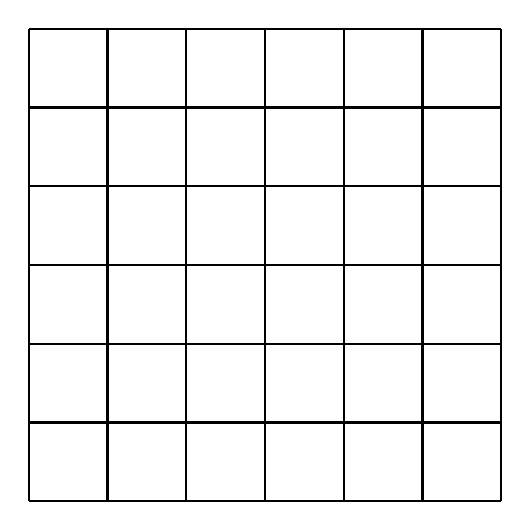
\begin{tikzpicture}[scale=1]
    \begin{scope}[thick,local bounding box=name]
    	\ColorCells{
    		1/1/brown/s, 2/1/brown/s, 3/1/brown/s, 4/1/brown/s, 5/1/brown/s, 6/1/brown/s,
    		1/2/brown/s, 2/2/white/30, 3/2/white/31, 4/2/white/32, 5/2/white/33, 6/2/brown/s,
    		1/3/brown/s, 2/3/white/20, 3/3/blue/21, 4/3/white/22, 5/3/white/23, 6/3/brown/s,
    		1/4/brown/s, 2/4/blue/10, 3/4/blue/11, 4/4/blue/12, 5/4/white/13, 6/4/brown/s,
    		1/5/brown/s, 2/5/white/00, 3/5/blue/01, 4/5/white/02, 5/5/white/03, 6/5/brown/s,
    		1/6/brown/s, 2/6/brown/s, 3/6/brown/s, 4/6/brown/s, 5/6/brown/s, 6/6/brown/s
    	}
    	\draw (0, 0) grid (\GridSize, \GridSize);
	\end{scope}
	\end{tikzpicture}
\caption{Example grid with fluid (blue), air (white) and solid (brown) cells\\
and a closed boundary.}\label{fig:grid-example}
\end{figure*}
\begin{figure*}
\centering
\[
	\begin{blockarray}{ccccccccccccccccc}
	& 00 & 01 & 02 & 03 & 10 & 11 & 12 & 13 & 20 & 21 & 22 & 23 & 30 & 31 & 32 & 33\\
	\begin{block}{c(cccccccccccccccc)}
		00 & \textcolor{red}{\text{-}2} & \textcolor{blue}{1} & & & \textcolor{blue}{1} & & & & & & & & & & &  \\
  		01 & \textcolor{blue}{0} & \textcolor{red}{\text{-}3} & \textcolor{blue}{0} & & & \textcolor{blue}{1} & & & & & & & & & & \\
	  	02 & & \textcolor{blue}{1} & \textcolor{red}{\text{-}3} & \textcolor{blue}{0} & & & \textcolor{blue}{1} & & & & & & & & & \\
  		03 & & & \textcolor{blue}{0} & \textcolor{red}{\text{-}2} & & & & \textcolor{blue}{0} & & & & & & & & \\
  		10 & \textcolor{blue}{0} & & & & \textcolor{red}{\text{-}3} & \textcolor{blue}{1} & & & \textcolor{blue}{0} & & & & & & & \\
  		11 & & \textcolor{blue}{1} & & & \textcolor{blue}{1} & \textcolor{red}{\text{-}4} & \textcolor{blue}{1} & & & \textcolor{blue}{1} & & & & & & \\
		12 & & & \textcolor{blue}{0} & & & \textcolor{blue}{1} & \textcolor{red}{\text{-}4} & \textcolor{blue}{0} & & & \textcolor{blue}{0} & & & & & \\
		13 & & & & \textcolor{blue}{0} & & & \textcolor{blue}{1} & \textcolor{red}{\text{-}3} & & & & \textcolor{blue}{0} & & & & \\
		20 & & & & & \textcolor{blue}{0} & & & & \textcolor{red}{\text{-}3} & \textcolor{blue}{1} & & & \textcolor{blue}{0} & & & \\
		21 & & & & & & \textcolor{blue}{1} & & & \textcolor{blue}{0} & \textcolor{red}{\text{-}4} & \textcolor{blue}{0} & & & \textcolor{blue}{0} & & \\
		22 & & & & & & & \textcolor{blue}{1} & & & \textcolor{blue}{1} & \textcolor{red}{\text{-}4} & \textcolor{blue}{0} & & & \textcolor{blue}{0} & \\
		23 & & & & & & & & \textcolor{blue}{0} & & & \textcolor{blue}{0} & \textcolor{red}{\text{-}3} & & & & \textcolor{blue}{0}  \\
		30 & & & & & & & & & \textcolor{blue}{0} & & & & \textcolor{red}{\text{-}2} & \textcolor{blue}{0} & & \\
		31 & & & & & & & & & & \textcolor{blue}{1} & & & \textcolor{blue}{0} & \textcolor{red}{\text{-}3} & \textcolor{blue}{0} & \\
		32 & & & & & & & & & & & \textcolor{blue}{0} & & & \textcolor{blue}{0} & \textcolor{red}{\text{-}3} & \textcolor{blue}{0}  \\
		33 & & & & & & & & & & & & \textcolor{blue}{0} & & & \textcolor{blue}{0} & \textcolor{red}{\text{-}2} \\
	\end{block}
	\end{blockarray}
	\cdot 
	\begin{blockarray}{c}
	\\
	\begin{block}{(c)}
		p_{0,0} \\
		p_{0,1} \\
		p_{0,2} \\
		p_{0,3} \\
		p_{1,0} \\
		p_{1,1} \\
		p_{1,2} \\
		p_{1,3} \\
		p_{2,0} \\
		p_{2,1} \\
		p_{2,2} \\
		p_{2,3} \\
		p_{3,0} \\
		p_{3,1} \\
		p_{3,2} \\
		p_{3,3} \\
	\end{block}
	\end{blockarray}
\]
\caption{Laplace Matrix \textbf{A} derived from Fig. \ref{fig:grid-example} with corresponding pressure vector.\\
Diagonal are marked as red, neighbors as blue (0 for air, 1 for fluid) and non neighbors are left out (0).}\label{fig:laplace-matrix}
\end{figure*}



